% !TEX program = lualatex
% !TEX root = main.tex
\documentclass[12pt,letterpaper]{article}
% Only practice placeholders. Replace these before producing a final paper.
\newcommand{\ContestYear}{2026}
\newcommand{\ProblemChosen}{Problem A}
\newcommand{\TeamNumber}{14013}
\newcommand{\PaperTitle}{基于双索引 SEIHFR 模型对本迪布焦型埃博拉疫情的数学建模}

% LuaLaTeX, compatible with Realtime TeX. No shell-escape required.
\usepackage[margin=1in,headheight=16pt]{geometry}
\usepackage{fontspec}
% Chinese support for LuaLaTeX / Realtime TeX; keep English headings unchanged.
\usepackage{luatexja-fontspec}
\setmainjfont{FandolSong-Regular.otf}[BoldFont=FandolSong-Bold.otf,ItalicFont=FandolKai-Regular.otf]
\setsansjfont{FandolHei-Regular.otf}[BoldFont=FandolHei-Bold.otf]
\setmonojfont{FandolFang-Regular.otf}
\setmainfont{TeX Gyre Termes}[Renderer=Basic]
\setsansfont{TeX Gyre Heros}[Renderer=Basic]
\setmonofont{TeX Gyre Cursor}[Renderer=Basic]
\usepackage{amsmath,amssymb}
\usepackage{unicode-math}
\setmathfont{TeX Gyre Termes Math}
\usepackage{graphicx}
\graphicspath{{figures/}{../results/}}
\usepackage{booktabs,array,longtable}
\usepackage{enumitem}
\usepackage{caption,subcaption}
\usepackage{xcolor}
\usepackage{fancyhdr,lastpage}
\usepackage{xurl}
\usepackage{tikz}
\usetikzlibrary{arrows.meta,positioning}
\usepackage[hidelinks]{hyperref}
\hypersetup{pdftitle={\PaperTitle},pdfauthor={},pdfsubject={MCM/ICM practice}}
\pagestyle{fancy}
\fancyhf{}
\fancyhead[L]{Team \# \TeamNumber}
\fancyhead[R]{Page \thepage\ of \pageref*{LastPage}}
\renewcommand{\headrulewidth}{0.4pt}
\setlength{\parindent}{1.5em}
\setlength{\parskip}{0.25em}
\setlist{nosep}
\numberwithin{equation}{section}
% 目录只到 subsection，避免 5.x.y 级条目把目录撑到两页。
\setcounter{tocdepth}{2}
% Chinese and English text are supported. Do not load xeCJK with LuaLaTeX.


\begin{document}
% Summary Sheet: keep this entire first page within ONE page.
\thispagestyle{empty}
\noindent
\begin{minipage}[t]{0.30\textwidth}
\centering Problem Chosen\\[6pt]
{\Large\bfseries \ProblemChosen}
\end{minipage}\hfill
\begin{minipage}[t]{0.34\textwidth}
\centering {\bfseries \ContestYear\\CQU MCM\\Summary Sheet}
\end{minipage}\hfill
\begin{minipage}[t]{0.30\textwidth}
\centering Team Control Number\\[6pt]
{\Large\bfseries \TeamNumber}
\end{minipage}
\par\vspace{8pt}\hrule\vspace{18pt}
\begin{center}
{\Large\bfseries \PaperTitle\par}
\vspace{12pt}
{\large\bfseries Summary}
\end{center}
% !TEX root = ../main.tex
本迪布焦型埃博拉疫情自 2026 年 5 月起在刚果（金）8 个省、66 个卫生区扩散，累计确诊约 10\,060 例、死亡约 4\,887 人，肯尼亚与尼日利亚已出现输入病例，题目要求我们从传播机制一直做到面向卫生部与国际捐助方的执行摘要。

任务一，我们建立含人际、院内与葬礼三条传播通道的双索引八舱连续时间模型（$S\to V\to E\to I\to H\to T\to F\to R$），以省与家庭双索引刻画省际流动，并用时变传播强度 $k(t)$ 描述干预随时间加强。

任务二，以 27 周全国序列、16 节点对数样条加二阶差分惩罚估计 $k(t)$ 与检出比例：样本内 $R^2=0.955$、RMSE $=34.6$ 例/周、MAPE $=6.9\%$，前 20 周拟合、后 7 周回测 RMSE $=119.5$、MAPE $=20.2\%$；得 $\theta=0.3382$、$\delta=0.486$、$\rho=0.392$，后期有效再生数为 0.893。

任务三，在统一情景口径下从第 27 周外推 26 周，基线新增 5\,672 例、报告口径死亡 2\,937 例。单措施中安全安葬最有效（2\,172 例，$-61.7\%$，30 周内收尾），接种 5\%/周为 2\,591 例（$-54.3\%$），院内感染控制 $-17.1\%$，治疗 50\% 为 4\,199 例（$-26.0\%$），而单独加快隔离与单独提高追踪率反而使新增增加 2.0\% 与 3.4\%。组合 C2 为 1\,834 例（$-67.7\%$）、C3 为 1\,590 例（$-72.0\%$）。若 7 月中旬即达到当前干预强度，同期末为 6\,884 例而非 17\,188 例，少 10\,303 例（$59.9\%$）与 4\,833 例死亡，收尾提前约 30 周。随访率由 78\% 提高到 90\%/95\%，26 周新增降至 5\,520/4\,720 例，需增约 3\,200/4\,600 名社区工作者与 6\,150/8\,700 万美元。

任务四，省际流动矩阵由重力先验加单参数标定；出行限制只改变空间分布与响应时间，不能单独压低全国总量。跨境不直接外推当地数值，而按 $R_{\mathrm{local}}\in\{0.8,1.0,1.2,1.5\}$ 判定：$R_{\mathrm{local}}\le 1$ 时输入链必然熄灭，1.2 时为 19\%--23\%，1.5 时为 3\%--4\%。

任务五，在传播强度 $\pm30\%$、检出比例 $\rho\in[0.30,0.50]$ 与干预时机联合扰动下，安葬优先于接种的排序不变，但有效再生数的结构性包络 $[0.62,1.22]$ 跨越 1，故不把“已确定低于 1”当作决策前提。

任务六，我们建议优先保障安全安葬和医院感染控制，并加强接触者追踪。对于超过 4 亿美元的资金缺口，国际援助不仅关系到当地救治，也关系到周边国家能否减少输入病例及后续防控支出。  
  
\noindent\rule{\linewidth}{0.4pt}
                                          
\noindent\textbf{关键词：}埃博拉病毒病；双索引SEIHFR 模型；时变参数；省际流动；下一代矩阵；干预组合优化；不确定性分析
\vfill
\clearpage

\tableofcontents
\clearpage
% !TEX root = ../main.tex
\section{Introduction}
\label{sec:introduction}

\subsection{Problem Background}

埃博拉病（Ebola virus disease, EVD）由埃博拉病毒引起，主要经直接接触感染者或病亡者的体液传播，病死率高。1976 年该病在扎伊尔（今刚果民主共和国）被首次识别，此后非洲已报告二十余次暴发；其中 2014--2016 年西非疫情的规模最大，报告病例超过 28\,000 例、死亡超过 11\,000 人\cite{whofactsheet,reliefweb2016}。

2026 年 5 月，刚果民主共和国再次暴发疫情。到 2026 年 10 月 25--26 日，本轮疫情已持续约五个月，累计确诊约 10\,060 例、累计死亡约 4\,887 人，粗病死率约 48.6\%，波及 8 个省的 66 个卫生区\cite{whodon622,ebolatrader}。本轮由本迪布焦病毒引起，与常见的扎伊尔毒株不同，目前尚无获批的疫苗或特异性治疗药物；世界卫生组织已在 5 月宣布本轮疫情构成国际关注的突发公共卫生事件\cite{whosituation2026}。

从公开通报看，防控的困难并不在单一环节。八成以上的新发病例是在已登记的接触者之外被发现的，说明现有追踪没有覆盖真实的传播面；约三分之二的死亡发生在社区，患者生前未在医疗机构就诊，说明葬礼和家庭内接触仍在传播中占有主要份额，不能只当作院内传播的补充。伊图里、北基伍等地武装冲突持续，治疗中心曾遭袭击，检测实验室从 1 家增加到 16 家、收治床位超过 800 张、接触者随访率接近 80\% 之后，世界卫生组织与非洲疾病预防控制中心的联合应对计划仍有超过 4 亿美元的资金缺口\cite{whodg2026}。境外方面，肯尼亚已报告 9 例确诊病例，尼日利亚于 10 月 20 日确诊首例，该病例有乌干达旅行史\cite{whodon622}。

\subsection{Problem Restatement and Task Breakdown}

题目要求围绕本轮疫情完成六件事。

\begin{enumerate}[label=\arabic*.,leftmargin=1.8em]
  \item 建立描述传播动力学的连续时间模型，逐条说明假设及其生物学或流行病学依据，给出完整常微分方程组并解释每一状态转移的机制与参数含义；模型要包含人际、院内和葬礼三条传播途径，并用时变参数反映干预强度的变化。
  \item 收集疫情数据，说明来源与预处理方法，估计关键参数，评价拟合优度，并讨论不确定性从何而来。
  \item 在第一个任务建立的模型上，逐项考察患者隔离、接触者追踪、安全安葬、院内感染控制、疫苗接种、MBP134/瑞德西韦治疗、奥贝德西韦暴露后预防和社区健康教育对累计病例、死亡人数与疫情持续时间的影响；比较若干组合方案；比较 7 月中旬（2\,073 例）即加强干预与现阶段（10\,060 例）才加强干预的差别；测算把随访率从 78\% 提高到 90\% 或 95\% 需要多少资源、又能减少多少传播。
  \item 建立空间传播模型，考虑省际人口流动矩阵、出行限制与边境管控、区域联防联控和环围疫苗接种，分析各种空间策略对扩散的影响，判断局部暴发在什么条件下会演变为大规模流行，并评估肯尼亚的 9 例输入和尼日利亚的首例是否可能引起持续的本地传播、应当采取什么措施。
  \item 做敏感性分析，找出对结果影响最大的参数，讨论数据质量、参数估计、毒株特性、冲突局势与人群行为变化带来的不确定性，检验模型在不同情景下的稳健性并说明局限。
  \item 面向刚果民主共和国卫生部与国际捐助方撰写执行摘要，交代背景，给出核心发现、最紧迫的行动建议、资源需求与资金缺口，并说明为什么这属于国家安全投资而不只是慈善。
\end{enumerate}

提交的 PDF 不超过 25 页，依次为单页摘要表、目录、正文（执行摘要可以并入）与参考文献；若使用人工智能，另附使用报告，不计入页数。

\subsection{Our Work}

本文的分析沿一条线推进：先把多层级通报数据整理成可以用于估计的周序列，在八舱连续时间模型上估计时变传播强度与检出比例，再把标定好的模型分别用于干预情景、空间与跨境、敏感性三个方向，最后汇总成执行摘要（图~\ref{fig:workflow}）。

\begin{figure}[htbp]
\centering
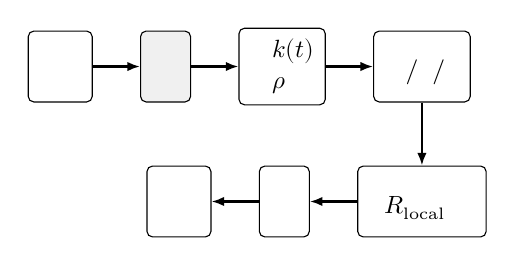
\begin{tikzpicture}[
  node distance=5mm and 6mm,
  box/.style={draw,rounded corners=2pt,align=center,font=\small,inner sep=4pt,minimum height=9mm},
  hub/.style={box,fill=black!6},
  arr/.style={-{Latex[length=1.6mm]},thick}
]
\node[box] (data) {通报数据\\三层口径分离};
\node[hub,right=of data] (model) {八舱连续\\时间模型};
\node[box,right=of model] (est) {样条 $k(t)$\\与 $\rho$ 估计};
\node[box,right=of est] (int) {干预情景\\单措施/组合/时机};
\node[box,below=8mm of int] (spa) {空间与跨境\\按 $R_{\mathrm{local}}$ 分情景};
\node[box,left=of spa] (sen) {敏感性\\参数包络};
\node[box,left=of sen] (pol) {执行摘要\\优先级与资金};
\draw[arr] (data) -- (model);
\draw[arr] (model) -- (est);
\draw[arr] (est) -- (int);
\draw[arr] (int) -- (spa);
\draw[arr] (spa) -- (sen);
\draw[arr] (sen) -- (pol);
\end{tikzpicture}
\caption{建模与交付的先后关系}
\label{fig:workflow}
\end{figure}

模型把社区、院内、葬礼三条通道写进同一个感染力，省与家庭两层索引分别承担人口流动与葬礼混合池的作用。这样处理的理由很直接：三条通道若各用一套参数，院内与葬礼传播的相对强弱就无从比较，"加快收治反而增加病例"这类结果在结构上根本不会出现。

参数估计使用 27 周全国序列，第 10 周的补报单独处理。时变强度取 16 节点对数样条加二阶差分惩罚，与检出比例一同估计，得到样本内 $R^2=0.955$、RMSE 为 34.6 例/周；用前 20 周拟合、后 7 周回测，RMSE 为 119.5、MAPE 为 20.2\%。检出比例估计为 0.392，后期有效再生数为 0.893。全文只保留这一套参数，摘要、正文和政策部分的数字都由它生成。

由此得到的主要结果如下。从第 27 周外推 26 周，基线新增 5\,672 例、报告口径死亡 2\,937 例；单措施中安全安葬最有效，累计病例降至基线的 $61.7\%$ 以下（30 周内收尾），接种 5\%/周与治疗次之，院内感染控制为 $-17.1\%$；四件套组合 C2 可减少 $67.7\%$，加入接种与治疗的 C3 减少 $72.0\%$。干预提前到 7 月中旬时，同期末病例由 17\,188 例降到 6\,884 例。有两处结果与直觉相反：单独加快隔离、单独提高追踪率会让 26 周新增分别增加 2.0\% 与 3.4\%，原因是标定得到的院内人均感染力约为社区的两倍，收治加快等于把病人更快送进更危险的舱室；出行限制改变的是空间分布和响应时间，压不下全国总量。前一点在组合情景中得到了反证，配上院内感染控制之后，同样的动作变为 $-20.0\%$。

不确定性没有压成单点数字。有效再生数同时给出条件统计区间 $[0.86,0.93]$ 与强度整体扰动 $\pm30\%$ 后的包络 $[0.62,1.22]$，后者跨过 1，因此下文不把"已经低于 1"当作既定前提。跨境风险也没有把刚果（金）的估计值直接推给邻国，而是按当地再生数取 0.8、1.0、1.2、1.5 四种情景分别判断：不超过 1 时输入链必然熄灭，1.2 时局部暴发概率为 19\%--23\%，1.5 时降至 3\%--4\%。

% !TEX root = ../main.tex
\section{Assumptions and Justifications}
\label{sec:assumptions}

\subsection{Model Basis}

埃博拉患者通常在出现症状后才具有传染性，病亡者的遗体仍可能造成感染，因此仅用易感、感染和康复三种状态（经典SIR模型）不足以区分疾病进程与救治情况\cite{whofactsheet}。Legrand 等人建立的 SEIHFR 模型将人群分为易感者（$S$）、潜伏者（$E$）、社区发病者（$I$）、住院患者（$H$）、死亡但尚未安葬者（$F$）以及已退出传播过程者（$R$），分别考虑社区、医院和葬礼中的传播\cite{legrand2007}。图~\ref{fig:seihfr-basis} 给出这一状态划分。

\begin{figure}[htbp]
\centering
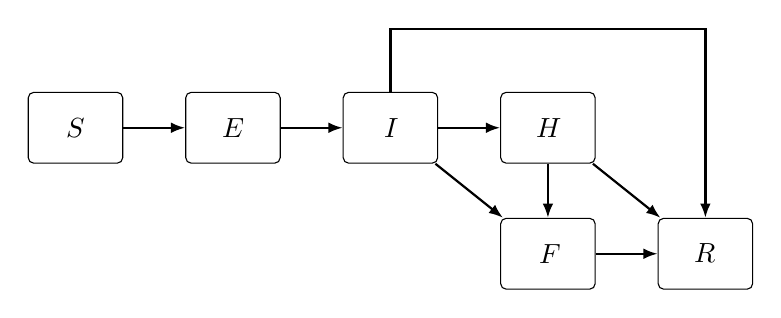
\begin{tikzpicture}[
  state/.style={draw,rounded corners=2pt,minimum width=12mm,minimum height=9mm},
  flow/.style={-{Latex[length=1.8mm]},thick}
]
\node[state] (s) at (0,0) {$S$};
\node[state] (e) at (2,0) {$E$};
\node[state] (i) at (4,0) {$I$};
\node[state] (h) at (6,0) {$H$};
\node[state] (f) at (6,-1.6) {$F$};
\node[state] (r) at (8,-1.6) {$R$};
\draw[flow] (s) -- (e);
\draw[flow] (e) -- (i);
\draw[flow] (i) -- (h);
\draw[flow] (i) -- (f);
\draw[flow] (h) -- (f);
\draw[flow] (f) -- (r);
\draw[flow] (h) -- (r);
\draw[flow] (i.north) -- ++(0,0.8) -| (r.north);
\end{tikzpicture}
\caption{基础 SEIHFR 模型的状态转移示意，依据文献\cite{legrand2007}重绘。$R$ 包含康复者与已安葬的死者；箭头表示状态转移，不表示传播途径。}
\label{fig:seihfr-basis}
\end{figure}

该模型采用人群均匀混合的近似，没有逐一描述家庭成员及家属尸体、医护人员和其他接触者之间的关系。Legrand 等人也指出，均匀混合可能不足以反映家庭接触对传播的影响\cite{legrand2007}。这属于模型对接触结构的简化，不能等同于数值模拟中的随机采样错误。对于本题，还需要区分患者所在地区及地区之间的人口流动，单一人群的汇总模型无法直接给出这些信息。

本文保留六种基础状态，以 $j$ 表示所在省份、$k$ 表示家庭型，记相应人数为 $X_{jk}(t)$，其中 $X\in\{S,E,I,H,F,R\}$。省份分为八组，家庭型按城乡分为两组。这里的“家庭型”是人口类别，不是一个具体家庭，也不代表已经获得了逐户的亲属关系数据。第二个索引用于保留组间差异，组内仍作平均化处理。接种与治疗情景另设 $V$、$T$ 两种状态；它们不是所有基线计算都必须包含的舱室。各状态的完整定义与方程组在后文模型建立部分给出。

\subsection{Assumptions}

\begin{enumerate}[label=\textbf{A\arabic*.},leftmargin=2.6em,itemsep=0.6em]

\item \textbf{人口分类互不重叠。}
同一时刻，每个人只计入一个省份、一种家庭型和一种疾病状态。短期出行只改变所在省份，不改变家庭型。这样可以避免在省际汇总时重复计数；研究期内发生的长期迁居或家庭型变化暂不单独处理。

\item \textbf{不计自然出生和非疫病死亡。}
模型关注本轮疫情及随后一段时间的变化，暂不考虑与疫情无关的人口增减。省际流动只改变各省的人口分布，不凭空增加或减少模型中的人数。疫情死亡仍须保留在状态转移和人口核算中，不能因忽略自然死亡而一并省略。

\item \textbf{潜伏者不参与传播，潜伏期结束后进入发病状态。}
这一处理与 WHO 关于症状出现前不传播疾病的说明一致\cite{whofactsheet}，也沿用了基础 SEIHFR 的潜伏状态定义。模型不另设无症状感染舱，因此不用于估计无症状感染的比例。

\item \textbf{康复者与已安葬的死者退出本模型描述的传播过程。}
二者均计入 $R$，但并不具有相同的医学含义。康复者在研究期内不再返回易感状态；对已完成安全处置的遗体，不再计算后续接触传播。这是短期模型的简化。WHO 提醒，部分康复者体内仍可能存在病毒，故不能把 $R$ 的数学定义解释为所有康复者均不存在后续传播风险\cite{whofactsheet}。

\item \textbf{组内接触采用均匀混合近似。}
社区和医院接触按所在省份汇总，葬礼接触则用家庭型分组表示。这样可以在缺少逐人接触记录时建立人口层面的模型，但同一家庭型中的人不一定互有亲属关系。因此，家庭型分组只是对接触差异的近似，不能据此声称模型已经还原了真实亲属网络。

\item \textbf{遗体不参与通常的人口流动。}
遗体留在死亡所在地对应的分组，直到完成安葬；其余状态在基础设定中使用相同的省际流动规则。后一个设定主要出于缺少分状态出行数据的限制，并不意味着住院患者与普通居民具有相同的出行能力。解释空间预测时须考虑这一简化，尤其不能把由此得到的外溢估计视为已观测事实。

\item \textbf{个体病程用舱室平均转移过程表示。}
模型不逐人记录感染、发病、入院和结局的具体日期，而以相应状态的平均停留过程描述人群变化。这使常微分方程模型可以使用汇总病例资料，但会忽略病程的个体差异。参数的取值依据与不确定范围放在参数估计部分说明，不将拟合所得的平均值当作每位患者共同遵循的病程。

\item \textbf{报告病例与模型中的感染人数分开处理。}
报告记录可能受到漏检、延迟上报和历史补录的影响，不能直接等同于同期发生的全部感染。参数估计时设置观测关系，并区分不同层级和统计日期。病例曲线中的突变既可能来自疫情变化，也可能来自记录方式变化，不能仅靠拟合曲线判定原因。

\item \textbf{干预效果和输入情况按情景给定。}
干预强度允许随时间变化，不在整个研究期内固定为同一水平。进行方案比较时，除明确改变的条件外，其余设定保持一致；跨境输入另行计入，不把省际系统封闭的近似套用于输入病例分析。比较结果表示给定条件下的模型差异，不等同于已经测得的政策因果效应。

\item \textbf{疫苗与治疗只作为假设性情景扩展。}
扩展模型中的 $V$ 表示已获得保护者，不能直接解释为所有已经接种的人；$T$ 表示接受相应治疗的住院患者。将接种者全部视为立即获得保护，是该扩展中的理想化设定。WHO 指出，针对本迪布焦病毒的疫苗与特异性治疗仍在研发中\cite{whofactsheet}，因此不能把情景中预设的保护或治疗效果写成已经证实的临床结论。

\end{enumerate}

上述假设中，症状出现前的传播性质有流行病学依据；家庭型划分、组内混合和统一流动规则则是受数据条件限制的建模选择。

% !TEX root = ../main.tex
\section{Notations}
\label{sec:notations}

本文使用的主要符号见表~\ref{tab:notations}。时间以周为单位，文献中按日给出的速率须先换算；比例在计算中取 $0$ 至 $1$，在结果中可写成百分数。除特别注明外，省份和家庭型下标在各状态变量中具有相同含义。

\begingroup
\setlength{\tabcolsep}{4pt}
\renewcommand{\arraystretch}{1.12}
\setlength{\LTleft}{0pt}
% Keep stretchable right glue for the longtable caption's zero-width box.
\setlength{\LTright}{0pt plus 1fill}
\begin{longtable}{@{}>{\raggedright\arraybackslash}p{0.23\linewidth}>{\raggedright\arraybackslash}p{0.62\linewidth}>{\raggedright\arraybackslash}p{0.09\linewidth}@{}}
\caption{主要符号及说明}\label{tab:notations}\\
\toprule
符号 & 含义 & 单位 \\
\midrule
\endfirsthead
\multicolumn{3}{l}{表~\thetable\quad 主要符号及说明（续）}\\
\toprule
符号 & 含义 & 单位 \\
\midrule
\endhead
\midrule
\multicolumn{3}{r}{续下页}\\
\endfoot
\bottomrule
\endlastfoot

\multicolumn{3}{@{}l}{\textbf{索引与时间}}\\*
$t$ & 连续时间，以研究起点为零点 & 周 \\
$i,j;\ J$ & 省份索引及省份总数；本文 $J=8$ & --- \\
$k;\ K$ & 家庭型索引及家庭型总数；本文按城乡分为两类，$K=2$ & --- \\
$n;\ n_{\mathrm{obs}}$ & 观测周的序号及参与当前拟合或验证的观测周数 & --- \\
$t_{\mathrm{int}},\ t_{\mathrm{end}}$ & 干预开始时刻与情景比较的共同终点 & 周 \\

\midrule
\multicolumn{3}{@{}l}{\textbf{状态变量与人口规模}}\\*
$X_{jk}(t)$ & 第 $j$ 省、第 $k$ 类家庭型中处于状态 $X$ 的人数；$X$ 为相应舱室的通用记号 & 人 \\
$S_{jk}(t)$ & 易感人数 & 人 \\
$E_{jk}(t)$ & 已感染但尚未进入发病状态的人数 & 人 \\
$I_{jk}(t)$ & 已发病、尚未住院的人数 & 人 \\
$H_{jk}(t)$ & 住院人数；在引入 $T$ 的扩展中，不含已计入 $T$ 的患者 & 人 \\
$F_{jk}(t)$ & 死亡但尚未安葬的人数，不是累计死亡人数 & 人 \\
$R_{jk}(t)$ & 已退出模型所描述传播过程的人数，包括康复者与已安葬的死者 & 人 \\
$V_{jk}(t)$ & 接种情景中已获得保护的人数，不等同于接种剂次数 & 人 \\
$T_{jk}(t)$ & 接受指定治疗的住院人数，与 $H$ 分开计数 & 人 \\
$N_j(t),\ M_k(t)$ & 第 $j$ 省与第 $k$ 类家庭型对应的人口规模；各自的计数范围须与模型分母的定义一致 & 人 \\

\midrule
\multicolumn{3}{@{}l}{\textbf{传播与病程参数}}\\*
$\lambda_{jk}(t)$ & 第 $j$ 省、第 $k$ 类家庭型中易感者的瞬时感染风险率 & 周$^{-1}$ \\
$\beta_I,\ \beta_H,$\newline $\beta_{F,k}$ & 社区、医院及第 $k$ 类家庭型葬礼接触的传播系数；不区分家庭型时记为 $\beta_F$ & 周$^{-1}$ \\
$h_{\mathrm{fac}}$ & 院内有效接触规模的折算因子；与医院传播项配套定义 & 无量纲 \\
$k(t)$ & 相对于基准传播系数的时变强度乘子，与家庭型下标 $k$ 区分 & 无量纲 \\
$\alpha$ & 潜伏状态向发病状态转移的速率参数 & 周$^{-1}$ \\
$\gamma_h,\ \gamma_d,\ \gamma_i$ & 与社区发病者入院、死亡及康复有关的病程速率参数；具体流出项还含相应分配系数 & 周$^{-1}$ \\
$\gamma_{dh},\ \gamma_{ih}$ & 与未进入指定治疗舱的住院患者死亡及康复有关的速率参数 & 周$^{-1}$ \\
$\gamma_{dt},\ \gamma_{it}$ & 与指定治疗舱内患者死亡及康复有关的速率参数 & 周$^{-1}$ \\
$\gamma_f$ & 未安葬状态向已安葬状态转移的速率参数 & 周$^{-1}$ \\
$\theta,\ \delta$ & 总体住院比例与最终死亡概率；$\delta$ 不直接等于任一报告日的粗病死率 & 无量纲 \\
$\theta_1$ & 将总体住院比例与病程速率对应起来的派生分配系数，不直接等于 $\theta$ & 无量纲 \\
$\delta_1,\ \delta_2,$\newline $\delta_{2t}$ & 分别用于社区、普通住院及指定治疗死亡流出项的派生系数；须结合竞争转移解释 & 无量纲 \\
$a$ & 计算派生分配系数时使用的病程辅助量 & 周$^{-1}$ \\
$\Delta,\ \Sigma_H,\ \Sigma_T$ & 离开社区发病、普通住院及指定治疗状态的总速率 & 周$^{-1}$ \\

\midrule
\multicolumn{3}{@{}l}{\textbf{干预与省际流动}}\\*
$\nu$ & 接种扩展中的转移速率；从接种到获得保护的假设在模型部分说明 & 周$^{-1}$ \\
$\phi$ & 入院患者中分配至指定治疗舱的比例 & 无量纲 \\
$\varepsilon$ & 治疗情景中预设的相对效果系数，作用对象由治疗参数化确定 & 无量纲 \\
$c_{\mathrm{follow}}$ & 接触者随访率，与检出比例 $\rho$ 区分 & 无量纲 \\
$W(t),\ w_{ij}(t)$ & 省际流动率矩阵及其元素；$w_{ij}$ 表示从省 $i$ 到省 $j$ 的人均流动率 & 周$^{-1}$ \\
$\mathcal{L}$ & 由省际流动率构成的净迁移算子；$\mathcal{L}X$ 表示状态 $X$ 的迁入与迁出净变化率 & 周$^{-1}$ \\
$G,\ \gamma_m$ & 归一化的省际流动相对权重矩阵与总体流动尺度；前者无量纲，后者为速率 & 见说明 \\
$m$ & 每周出省比例；用于离散时间描述时，不与连续时间流动率直接混用 & 无量纲 \\

\midrule
\multicolumn{3}{@{}l}{\textbf{观测与参数估计}}\\*
$\rho(t)$ & 感染或发病事件进入报告数据的观测比例；采用常数近似时记为 $\rho$ & 无量纲 \\
$\rho_{\max}$ & 检出比例参数化中的上限或渐近水平，不表示实际观测到的最大值 & 无量纲 \\
$t_0,\ r$ & 检出比例变化的过渡中心与变化速率；单位分别为周与周$^{-1}$ & 见说明 \\
$y_n,\ \widehat y_n$ & 第 $n$ 周的报告新增病例数与模型给出的对应预测值 & 例 \\
$C(t),\ C^{\mathrm{rep}}(t)$ & 模型累计发病数与报告累计病例数，二者不能与单周新增混用 & 例 \\
$D(t),\ D^{\mathrm{rep}}(t)$ & 模型累计死亡数与报告累计死亡数，二者采用的统计口径分别说明 & 人 \\
$\eta$ & 时变强度拟合的平滑惩罚权重；本文另用此记号，避免与感染风险率 $\lambda_{jk}$ 混淆 & 见说明 \\

\midrule
\multicolumn{3}{@{}l}{\textbf{再生数、输入风险与评价指标}}\\*
$\mathcal{F},\ \mathcal{V}$ & 在相应分析状态下线性化得到的新感染与其余转移矩阵；花体符号不指代舱室 $F,V$ & 周$^{-1}$ \\
$\mathcal{K}$ & 下一代矩阵 & 无量纲 \\
$R_0$ & 基本再生数，在规定的全易感基准状态下定义 & 无量纲 \\
$R_{\mathrm{eff}}(t)$ & 随易感状态与干预条件变化的有效再生数 & 无量纲 \\
$R_{\mathrm{local}},\ R_j$ & 输入地区的当地再生数与第 $j$ 省的再生数 & 无量纲 \\
$q$ & 指定分支过程下，一条输入传播链最终消退的概率，不是暴发概率 & 无量纲 \\
$R^2$ & 拟合的决定系数，与移出状态 $R$ 及再生数区分 & 无量纲 \\
$\mathrm{RMSE}$ & 均方根误差，与所比较的观测量同单位；本文用于周新增病例 & 例 \\
$\mathrm{MAPE}$ & 平均绝对百分比误差；百分数形式报告，零观测值的处理须另行说明 & \% \\
$\mathrm{CFR}$ & 同一报告口径下的粗病死率，不等同于个体最终死亡概率 & \% \\
$\mathrm{LHS},\ \mathrm{PRCC}$ & 拉丁超立方抽样与偏秩相关系数；前者为抽样方法，后者为无量纲统计量 & --- \\

\end{longtable}
\endgroup

状态变量中的下标省略时，须说明表示某一分组还是对各组求和。参考材料中与病程速率有关的 $g_h,g_d,g_i$ 等记号，在本文统一写为对应的 $\gamma$ 形式；流动尺度另记为 $\gamma_m$。粗体或花体的矩阵符号与同名舱室分开使用。

表中的 $y_n$ 是一周内的病例计数，因此 RMSE 以“例”计；若将输入数据写成每周平均发病速率，RMSE 才相应以“例/周”计。$C$ 与 $D$ 仅用于累计量。平滑权重 $\eta$ 的量纲随拟合目标的归一化方式确定，在参数估计部分给出。

% !TEX root = ../main.tex
\section{Data Description and Preprocessing}
\label{sec:data}

\subsection{Data Sources and Description}

本文使用题面统计及参考资料提供的 Ebola Tracker 病例数据库副本\cite{eboladatabase}。数据覆盖 2026 年 5 月 14 日至 11 月 17 日，共 9\,863 条记录，涉及 8 个省、68 个卫生区。其中，国家级记录 183 条、省级记录 994 条、卫生区级记录 8\,686 条。全国病例序列取自国家级记录，省级与卫生区级记录用于地区比较，三个层级不重复累加。题面统计截至 10 月下旬，与本文数据的截止日期不同。

研究起点已有确诊病例 8 例、死亡 4 人；截至末次报告，累计确诊 11\,613 例、死亡 5\,678 人。因此，研究期内新增确诊为 11\,605 例，新增死亡为 5\,674 人，二者分别与新增字段的合计一致。

\subsection{Data Cleaning}

按日期、层级和地区检查后，未发现重复记录。缺失值不填零，也不对缺报日期插值；一次覆盖多日的新增记录仍归入报告日。累计病例字段完整，但国家级社区死亡和检测样本字段的缺失率分别为 34.97\% 和 26.78\%，卫生区级检测与随访字段则全部缺失，故不据此估计区级检测能力或随访情况。

对累计数的历史下调保留原记录，不强行修成单调序列。比较各区末期规模时，统一使用截止日的累计值，而非历史峰值。所附周表的累计死亡列误用了累计病例数据，本文改由国家级明细重建累计量，起始病例与期间新增分开计算。

死亡周序列还存在一项待核对差异：按明细报告日期汇总，第 25、26 周新增死亡分别为 241、238 人，所附周表则为 346、133 人。两者总量相同，周次分配相差 105 人。本文暂按明细报告日汇总；使用原周表得到的死亡拟合结果仍需复核。

\subsection{Feature Processing}

以 5 月 14 日为起点，每 7 天划分一个左开右闭区间，将国家级新增记录按报告日期求和，得到 27 周序列。第 $n$ 周的新增病例记为 $y_n$，各周合计为 11\,605 例。最后一个区间截至 11 月 19 日，而数据只到 11 月 17 日，因此末周并不完整。

第 10 周报告新增 792 例，其中 7 月 22 日有 369 例被标记为补报，占该周的 46.6\%。本文保留这一周并注明补报情况，不将全部峰值解释为同期传播加快。周序列描述的是报告时间分布，不等同于真实发病时间分布。

病死率由同一层级、同一日期的累计死亡与累计病例计算；随访率仅在分子、分母统计期一致且记录可用时计算。回测按时间划分为前 20 周拟合、后 7 周检验，参数选择不使用验证期数据。病例资料不含逐户接触关系或实际人口流动记录，这些信息需由其他资料或模型假设补充。

% !TEX root = ../main.tex
\section{Model Development and Solution}
\label{sec:model}

% !TEX root = ../../main.tex
\subsection{Task 1: Continuous-Time Model}
\label{sec:task-1}

\subsubsection{Population Groups and Contact Structure}

在 Legrand 等人的六状态框架\cite{legrand2007}中，以 $j$ 表示省份、$k$ 表示家庭型。取 $J=8$、$K=2$，系统共含 96 个状态变量。各组记账人口及其汇总量为
\begin{equation}
N_{jk}(t)=\sum_{X\in\{S,E,I,H,F,R\}}X_{jk}(t),\qquad
N_j(t)=\sum_{k=1}^{K}N_{jk}(t),\qquad
M_k(t)=\sum_{j=1}^{J}N_{jk}(t).
\label{eq:group-population}
\end{equation}
记账人口包含已移出者；在接种和治疗情景中，求和相应加入 $V,T$。

省内社区、医院接触按省汇总，葬礼接触限定在同省、同家庭型中：
\begin{equation}
\lambda_{jk}(t)=k(t)\left[
\beta_I\frac{\sum_{\ell=1}^{K}I_{j\ell}}{N_j}
+\beta_H\frac{\sum_{\ell=1}^{K}H_{j\ell}}{h_{\mathrm{fac}}N_j}
+\beta_{F,k}\frac{F_{jk}}{N_{jk}}
\right].
\label{eq:infection-pressure}
\end{equation}
其中 $k(t)$ 为时变强度乘子，$h_{\mathrm{fac}}$ 折算院内接触规模，$\ell$ 为求和下标。$M_k$ 用于跨省汇总；人口为零的组，其接触项取零。

省际净迁移定义为
\begin{equation}
(\mathcal{L}X)_{jk}
=\sum_{i\ne j}w_{ij}(t)X_{ik}
-X_{jk}\sum_{i\ne j}w_{ji}(t).
\label{eq:migration-operator}
\end{equation}
$w_{ij}$ 为从 $i$ 省到 $j$ 省的速率。迁移作用于 $S,E,I,H,R$；$F$ 保留在死亡所在地。

\subsubsection{State Transitions}

社区发病者的入院、死亡和康复构成竞争转移。由住院比例 $\theta$ 与最终死亡概率 $\delta$ 定义
\begin{align}
\delta_1&=\frac{\delta\gamma_i}{\delta\gamma_i+(1-\delta)\gamma_d},
& a&=\gamma_d\delta_1+\gamma_i(1-\delta_1),\notag\\
\theta_1&=\frac{\theta a}{\theta a+(1-\theta)\gamma_h},
& \delta_2&=\frac{\delta\gamma_{ih}}{\delta\gamma_{ih}+(1-\delta)\gamma_{dh}},
\label{eq:probability-coefficients}\\
\Delta&=\gamma_h\theta_1+(1-\theta_1)a,
& \Sigma_H&=\gamma_{dh}\delta_2+\gamma_{ih}(1-\delta_2).
\label{eq:exit-rates}
\end{align}
在参数固定时，这些定义满足
\begin{equation}
\frac{\gamma_h\theta_1}{\Delta}=\theta,\qquad
\frac{\gamma_d\delta_1}{a}=\delta,\qquad
\frac{\gamma_{dh}\delta_2}{\Sigma_H}=\delta.
\label{eq:branch-probabilities}
\end{equation}
基线中住院和未住院两组共用 $\delta$；参数时变时，上式按当前冻结参数解释。

对每个 $(j,k)$，完整基础方程为
\begin{equation}
\left\{\begin{aligned}
\dot S_{jk}&=-\lambda_{jk}S_{jk}+(\mathcal{L}S)_{jk},\\
\dot E_{jk}&=\lambda_{jk}S_{jk}-\alpha E_{jk}+(\mathcal{L}E)_{jk},\\
\dot I_{jk}&=\alpha E_{jk}-\Delta I_{jk}+(\mathcal{L}I)_{jk},\\
\dot H_{jk}&=\gamma_h\theta_1I_{jk}-\Sigma_H H_{jk}+(\mathcal{L}H)_{jk},\\
\dot F_{jk}&=\gamma_d(1-\theta_1)\delta_1I_{jk}
             +\gamma_{dh}\delta_2H_{jk}-\gamma_fF_{jk},\\
\dot R_{jk}&=\gamma_i(1-\theta_1)(1-\delta_1)I_{jk}
             +\gamma_{ih}(1-\delta_2)H_{jk}\\
            &\quad+\gamma_fF_{jk}+(\mathcal{L}R)_{jk}.
\end{aligned}\right.
\label{eq:baseline-ode}
\end{equation}
$S\to E$、$E\to I$、$I\to H$ 分别表示感染、发病和住院；死亡者经 $F$ 安葬后进入 $R$，康复者直接进入 $R$。

相应的累计发病与累计死亡满足
\begin{align}
\dot C(t)&=\alpha\sum_{j,k}E_{jk}(t),\notag\\
\dot D(t)&=\sum_{j,k}\left[
\gamma_d(1-\theta_1)\delta_1I_{jk}
+\gamma_{dh}\delta_2H_{jk}\right].
\label{eq:cumulative-flows}
\end{align}
\subsubsection{Conservation and Reproduction Numbers}

数值求解采用自适应步长积分，在干预切换时刻衔接前一段末态；初始人数按疾病状态分配。

再生数采用下一代矩阵法\cite{diekmann1990,vandendriessche2002}。将全部组的 $E,I,H,F$ 排成感染相关状态向量，分别构造新感染矩阵 $\mathcal{F}$ 和其余转移矩阵 $\mathcal{V}$，则
\begin{equation}
\mathcal{K}=\mathcal{F}\mathcal{V}^{-1},\qquad
R_0=\operatorname{spr}(\mathcal{K})\big|_{\text{全易感基准状态}}.
\label{eq:next-generation}
\end{equation}
$\operatorname{spr}$ 表示谱半径，$\mathcal{V}$ 包含省际迁移。采用当前易感人数并冻结当前参数，可得 $R_{\mathrm{eff}}(t)$。

各状态转移成对计入，迁入与迁出相互抵消。非负初值下系统保持非负，并满足
\begin{equation}
\frac{\mathrm d}{\mathrm dt}\sum_{j,k}N_{jk}(t)=0,
\label{eq:population-conservation}
\end{equation}
式~\eqref{eq:population-conservation}作为积分结果的守恒检验。两类家庭的状态比例与参数相同时，分组系统退化为合并模型。

% !TEX root = ../../main.tex
\subsection{Task 2: Observation and Parameter Estimation}
\label{sec:task-2}

\subsubsection{Observation Model}

第 $n$ 周的报告新增预测及报告累计量分别为
\begin{align}
\widehat y_n&=\int_{n-1}^{n}\rho(t)\,\alpha\sum_{j,k}E_{jk}(t)\,\mathrm dt,
\label{eq:weekly-observation}\\
C^{\mathrm{rep}}(t)&=8+\int_0^t\rho(u)\dot C(u)\,\mathrm du.
\label{eq:reported-cumulative}
\end{align}
末周的积分上限取实际截止时间。周病例用于估计总体强度 $k(t)$ 与初始状态，病程参数和报告比例作为外部约束。

\subsubsection{Parameterization and Estimation}

在节点 $\tau_\ell$ 间对 $\log k(t)$ 作线性插值，最小化加权残差与节点二阶差分惩罚：
\begin{equation}
\begin{split}
\min\quad &\sum_{n=1}^{n_{\mathrm{obs}}}
\frac{(\widehat y_n-y_n)^2}{y_n+1}\\
&+\eta\sum_{\ell=2}^{L-1}
\left[\log k(\tau_{\ell+1})-2\log k(\tau_\ell)
+\log k(\tau_{\ell-1})\right]^2.
\end{split}
\label{eq:fitting-objective}
\end{equation}
$L$ 为节点数；病例以“1 例”为单位数值化，$\eta$ 为无量纲权重。采用有界非线性最小二乘，正值参数在对数尺度上估计，概率参数限于 $[0,1]$。多初值计算用于检验局部最优。

参考计算的全样本拟合使用 27 周数据和 16 个节点；时间回测仅用前 20 周及 11 个节点拟合，随后固定末节点强度预测第 21--27 周。评价指标为
\begin{align}
R^2&=1-\frac{\sum_n(y_n-\widehat y_n)^2}
{\sum_n(y_n-\overline y)^2},\notag\\
\mathrm{RMSE}&=\sqrt{\frac{1}{n_{\mathrm{obs}}}
\sum_n(y_n-\widehat y_n)^2},\qquad
\mathrm{MAPE}=\frac{100\%}{n_{\mathrm{obs}}}
\sum_n\frac{|y_n-\widehat y_n|}{y_n}.
\label{eq:fit-metrics}
\end{align}
$\overline y$ 为评价区间的观测均值，RMSE 以例计。当前周观测均为正，MAPE 无零分母。

\subsubsection{Fit and Temporal Validation}

根据所给参考预测序列重算得到表~\ref{tab:fit-audit}。全样本 $R^2=0.955$，但验证段 RMSE 为训练段的 3.61 倍，外推误差明显增加。

\begin{table}[!htbp]
\centering
\caption{参考预测序列的拟合与回测误差}
\label{tab:fit-audit}
\begin{tabular}{@{}lrrr@{}}
\toprule
评价区间 & $R^2$ & RMSE（例） & MAPE \\
\midrule
全样本拟合（1--27 周） & 0.955 & 34.61 & 6.90\% \\
回测训练段（1--20 周） & 0.969 & 33.09 & 6.96\% \\
回测验证段（21--27 周） & $-4.577$ & 119.50 & 20.15\% \\
\bottomrule
\end{tabular}
\end{table}

\begin{figure}[!htbp]
\centering
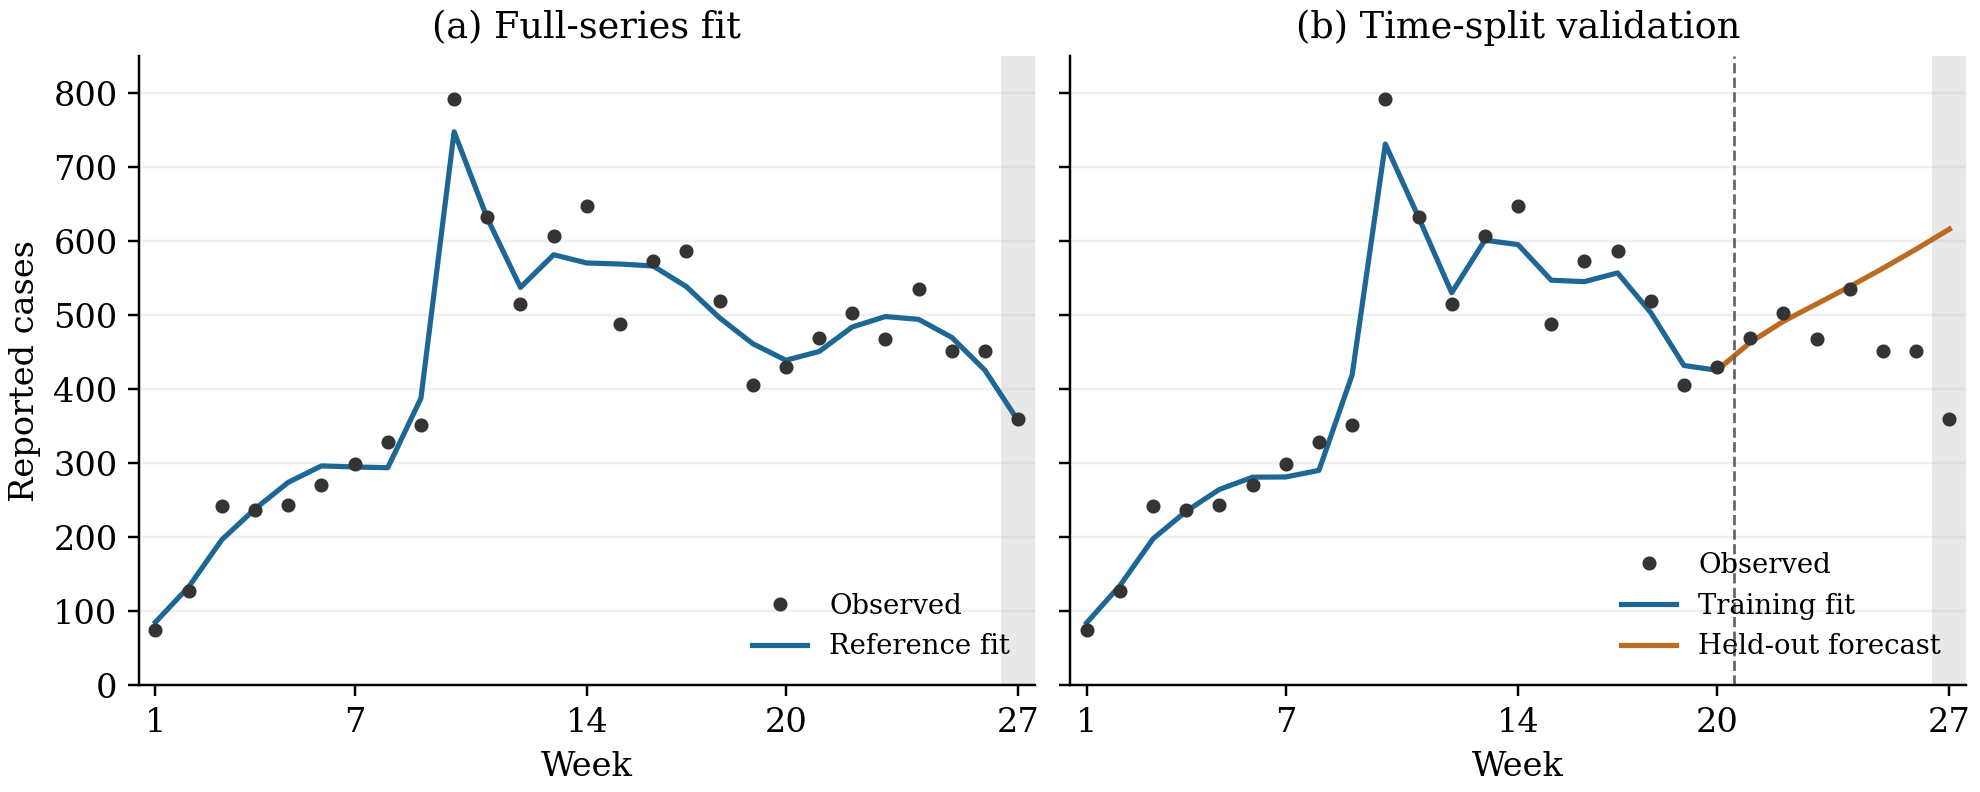
\includegraphics[width=0.94\linewidth]{model-fit-check.png}
\caption{参考计算的全样本拟合（左）与时间回测（右）；灰色区域为未完整覆盖的第 27 周，虚线为训练与验证分界。}
\label{fig:model-fit-check}
\end{figure}

全样本预测新增合计为 11\,517 例，观测合计为 11\,605 例。回测末周预测 616 例、记录 359 例；验证段 $R^2<0$，表明其平方误差超过以该段观测均值作常数对照的误差。末周覆盖及平滑权重的影响在第~\ref{sec:sensitivity} 节分析。

% !TEX root = ../../main.tex
\subsection{Task 3}
\label{sec:task-3}
test

\subsubsection{Problem Analysis}
test

\subsubsection{Model Formulation}
test

\subsubsection{Solution Method}
test

\subsubsection{Results and Interpretation}
test

% !TEX root = ../../main.tex
\subsection{Task 4: Spatial Spread and Cross-Border Risk}
\label{sec:task-4}

\subsubsection{Provincial Mobility}

将省际流动分解为总体尺度和相对流向：
\begin{equation}
w_{ij}(t)=\gamma_m(t)G_{ij},\qquad
G_{ii}=0,\quad G_{ij}\geq0,\quad
\sum_{j\ne i}G_{ij}=1.
\label{eq:mobility-scale}
\end{equation}
$G$ 为给定流动权重，$\gamma_m$ 为连续时间速率。若离省事件具有恒定速率，一周内至少离省一次的概率 $m$ 满足
\begin{equation}
\gamma_m=\frac{-\log(1-m)}{1\,\text{周}}.
\label{eq:rate-probability}
\end{equation}
流动改变各地易感者与感染者的分布，其总体影响由 $\sum_{j,k}\lambda_{jk}S_{jk}$ 决定。仅在参数及状态比例均质等条件下，全国累计量才可能对流动变化保持不变。

\subsubsection{Regional Control Strategies}

出行限制通过调整 $W(t)$ 表示；区域联防同时改变相邻地区的发现、转诊与院内防护条件。比较指标包括分省累计病例、首次报告时间及全国总量，并保持各方案的观测口径与评价终点一致。

环围接种以病例接触者及其接触者为目标，需要在病例关联资料上分配保护状态 $V$。现有省份与家庭型分组适于地区尺度比较，接触链层面的资源分配另需接触网络数据。

\subsubsection{Transmission Threshold and Imported Chains}

省际耦合系统的传播阈值由式~\eqref{eq:next-generation}确定。境外输入采用当地条件对应的 $R_{\mathrm{local}}$。设继发病例数服从几何分布，则单条输入链最终消退的概率为
\begin{equation}
q=\begin{cases}
1,&R_{\mathrm{local}}\leq1,\\
1/R_{\mathrm{local}},&R_{\mathrm{local}}>1.
\end{cases}
\label{eq:chain-extinction}
\end{equation}
采用泊松继发分布时，$q$ 则为 $q=\exp[R_{\mathrm{local}}(q-1)]$ 在 $[0,1]$ 内的最小解。$R_{\mathrm{local}}>1$ 时存在持续传播的可能；亚临界条件下，有限输入链最终消退。

题面给出的肯尼亚 9 例与尼日利亚 1 例是累计病例数。当地风险评估还取决于独立输入次数、当前活动病例及接触者调查结果。两国的应对重点是及时发现、规范收治、接触者随访和跨境信息共享，并据后续调查更新当地传播条件。


% !TEX root = ../main.tex
\section{Sensitivity Analysis}
\label{sec:sensitivity}
test

% !TEX root = ../main.tex
\section{Model Evaluation}
\label{sec:evaluation}

\subsection{Strengths}

模型在统一人口核算下区分社区、医院和葬礼接触，并将发病、死亡与报告过程分开。竞争转移系数具有明确的概率含义，接种与治疗扩展保持基础系统的非负性和守恒关系。时间回测与持续性基准共同评价外推性能，避免以样本内拟合替代预测检验。

\subsection{Limitations}

现有资料缺少逐户接触网络、实测省际流动及分组病程记录，限制了家庭型差异、流动矩阵和各接触系数的独立识别。$R$ 合并康复者与已安葬者，其迁移属于记账人口分配；住院者与普通居民共用流动规则也是空间近似。

数值评价目前基于参考病例预测。本文修正了竞争转移、接触范围和治疗参数化，修正系统仍需重新标定，再统一计算干预病例、死亡和持续时间。病例报告比例与死亡报告过程分别估计，药物和疫苗的效力依据相应临床证据更新。

后续验证应优先使用发病日期、入院时间、结局和跨地区转诊资料，并以滚动窗口检验外推误差。冲突与服务中断下的预测采用情景区间，而非单一路径。

% !TEX root = ../main.tex
\section{Conclusion}
\label{sec:conclusion}

本文构建省份与家庭型双索引的六状态模型，并以保护和治疗状态扩展干预机制。模型区分发病量、报告量与死亡量，在统一人口核算下描述省际流动。

参考预测的样本内 $R^2$ 为 0.955，后七周回测 RMSE 为 119.50 例；剔除未完整末周后仍高于持续性基准。相比平滑权重，报告比例和外推条件对结果解释更为关键。防控比较应统一起点、终点与统计口径，并结合地区服务能力更新。

建议将及时发现、规范收治、院内防护、安全安葬和接触者随访联合实施，按实际服务量编制资源预算。跨境应对以当地调查和区域信息共享为基础，疫苗与治疗情景随临床证据更新。

% !TEX root = ../main.tex
% thebibliography 自带“References”标题，这里只补目录条目，避免标题重复。
\addcontentsline{toc}{section}{References}
\begin{thebibliography}{99}
\small

\bibitem{whofactsheet}
World Health Organization. Ebola disease (fact sheet) [EB/OL].
\url{https://www.who.int/news-room/fact-sheets/detail/ebola-disease},
2026-11-21.

\bibitem{reliefweb2016}
ReliefWeb. 2014--2016 Ebola outbreak in West Africa [EB/OL].
\url{https://reliefweb.int/report/democratic-republic-congo/2014-2016-ebola-outbreak-west-africa},
2026-11-21.

\bibitem{whodon622}
World Health Organization. Disease Outbreak News: Ebola disease caused by Bundibugyo virus in the Democratic Republic of the Congo, Kenya and Nigeria [EB/OL].
\url{https://www.who.int/emergencies/disease-outbreak-news/item/2026-DON622},
2026-11-21.

\bibitem{whosituation2026}
World Health Organization. Ebola outbreak in the Democratic Republic of the Congo, 2026 [EB/OL].
\url{https://www.who.int/emergencies/situations/ebola-outbreak---drc-2026},
2026-11-21.

\bibitem{ebolatrader}
Ebola Tracker. Case data by province [EB/OL].
\url{https://ebola-tracker.org/en/data/?province=Ituri},
2026-11-21.

\bibitem{eboladatabase}
Ebola Tracker. Ebola DRC database [DS/OL].
\url{https://ebola-tracker.org/data/ebola-drc-database.csv}.
本文使用参考资料提供的本地副本，记录日期为 2026-05-14 至 2026-11-17；文件内附各条记录的原始通报链接。

\bibitem{whodg2026}
World Health Organization. WHO Director-General's opening remarks at the media briefing, 12 August 2026 [EB/OL].
\url{https://www.who.int/news-room/speeches/item/who-director-general-s-opening-remarks-at-the-media-briefing---12-august-2026},
2026-11-21.

\bibitem{insp2026}
Institut National de Sant\'e Publique, R\'epublique D\'emocratique du Congo. Weekly epidemiological reports on Ebola virus disease, 2026 [R]. Kinshasa: INSP, 2026.

\bibitem{legrand2007}
Legrand J, Grais R F, Boelle P Y, Valleron A J, Flahault A. Understanding the dynamics of Ebola epidemics [J]. Epidemiology and Infection, 2007, 135(4): 610--621.
\url{https://doi.org/10.1017/S0950268806007217}.

\bibitem{diekmann1990}
Diekmann O, Heesterbeek J A P, Metz J A J. On the definition and the computation of the basic reproduction ratio $R_0$ in models for infectious diseases in heterogeneous populations [J]. Journal of Mathematical Biology, 1990, 28(4): 365--382.
\url{https://doi.org/10.1007/BF00178324}.

\bibitem{vandendriessche2002}
van den Driessche P, Watmough J. Reproduction numbers and sub-threshold endemic equilibria for compartmental models of disease transmission [J]. Mathematical Biosciences, 2002, 180(1--2): 29--48.
\url{https://doi.org/10.1016/S0025-5564(02)00108-6}.

\end{thebibliography}


% Appendix: supplementary material, not a substitute for core arguments.
% Comment out this group if no appendix is needed; it counts toward the page limit.
\clearpage
\appendix
% !TEX root = ../main.tex
\section{Supplementary Material}
\label{sec:appendix}
test

\subsection{Code}
test

\subsection{Supplementary Tables}
test

\subsection{Derivations}
test


% Memo / Letter: enable when explicitly required by the chosen problem.
% Kept on a separate page, outside the main analysis and Summary.
% \clearpage
% % !TEX root = ../main.tex
\section*{Executive Summary}
\addcontentsline{toc}{section}{Executive Summary}
\label{sec:executive-summary}

\noindent\textbf{致：刚果民主共和国卫生部及国际捐助方}

\medskip
按题面统计，截至 2026 年 10 月 25--26 日，本轮疫情累计确诊约 10\,060 例、死亡约 4\,887 人，已波及 8 个省，肯尼亚与尼日利亚出现输入病例。社区发现不足、医疗服务受冲突影响和资金短缺共同制约疫情应对。

\paragraph{主要发现。}
研究资料延续至 11 月 17 日，期间新增确诊合计为 11\,605 例。参考病例预测能描述历史走势，但后七周回测 RMSE 为 119.50 例，高于持续性基准的 60.10 例；预测须随新增资料滚动更新。省际人口守恒并不保证传播总量不变，地区间的发现和救治能力应与流动情况同时评估。

\paragraph{近期行动。}
将病例发现、规范收治、院内防护、安全安葬与接触者随访作为连续服务组织实施。优先保障一线防护物资、转诊交通和安葬服务的可达性；对受冲突影响的地区，与当地社区协调服务安排和人员安全。追踪质量以实际随访、症状发现至转诊的时间及失访情况评价。

\paragraph{资源与资金。}
若以 2.1 万人为等效随访人力基数且人均工作量不变，随访率从 78\% 提至 90\% 或 95\%，对应新增约 3\,231 人或 4\,577 人。预算须结合专职投入、工作周期、交通与安全成本核定。题面所列超过 4 亿美元的应对资金缺口，应按可核验的人员、物资和服务项目分配，并定期公布资金执行与服务覆盖情况。

\paragraph{区域协作。}
建立跨境病例信息与转诊协作机制，及时共享病例关联和接触者调查结果。肯尼亚和尼日利亚的响应依据当地传播条件调整，持续监测输入后的病例发现和服务能力。针对本迪布焦病毒的疫苗及特异性治疗，按临床试验和监管进展更新应用安排。

\paragraph{对国家安全的投资。}
当地救治和监测能力的提升，有助于减少跨境输入、医疗挤兑及后续应急支出，并维持人员往来和基本公共服务。国际支持的收益超出单一国家，因此稳定的区域防控投入既具有公共卫生价值，也关系到周边国家的社会与经济安全。


% Optional separate disclosure, following the rules of the chosen problem.
% \clearpage
% % !TEX root = ../main.tex
\section*{Report on Use of AI}
\addcontentsline{toc}{section}{Report on Use of AI}

本文使用生成式 AI 编程助手，在 Pi 环境中辅助资料整理、章节组织、中文表述、符号统一及 LaTeX 排版。辅助检查包括原始数据汇总、保存预测序列的误差重算、方程守恒与概率关系的符号验证，以及编译和版面检查。

模型重构后的完整参数标定、干预模拟和空间情景计算尚未完成。文中的参考预测与新增统计检查分别标明来源和用途。本次新增统计来自现有数据与预测文件的计算。

本报告依题目要求单列，不计入解答正文的 25 页上限。

\end{document}
